\problema{4}{Difusión 1D con condiciones de Dirichlet}{8}

\begin{enunciado}
	Resuelva $-D\varphi'' + \Sigma_a \varphi = S$ en $0 < x < L$, con $\varphi(0) = \varphi(L) = 0$,
	$L = 10$, $D = 1$, $\Sigma_a = \tfrac12$, $S = 1$ y $h = 2$ (cuatro nodos interiores).
	
	\begin{center}
		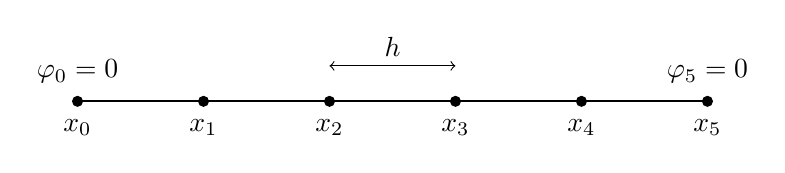
\begin{tikzpicture}[x=1.6cm]
			\draw[thick] (0,0) -- (5,0);
			\foreach \i in {0,...,5} {
				\fill (\i,0) circle (2pt);
				\node[below=3pt] at (\i,0) {$x_{\i}$};
			}
			\node[above=3pt] at (0,0) {$\varphi_0 = 0$};
			\node[above=3pt] at (5,0) {$\varphi_5 = 0$};
			\draw[<->] (2,0.45) -- node[above] {$h$} (3,0.45);
		\end{tikzpicture}
	\end{center}
	
	\begin{enumerate}[label=(\alph*)]
		\item Deduzca la ecuación discreta del nodo interior $i$ y su error de truncamiento.
		\item Escriba el sistema $\mat{A}\vect{\varphi} = \vect{b}$ y verifique que $\mat{A}$ es simétrica definida positiva.
		\item Obtenga la factorización de Gauss $\mat{A} = \mat{L}\mat{U}$.
		\item Obtenga la factorización triple $\mat{A} = \mat{L}\mat{D}\mat{L}^T$ y compare con (c).
		\item Obtenga la factorización de Cholesky $\mat{A} = \mat{G}\mat{G}^T$.
		\item Resuelva el sistema con la factorización de su elección y verifique con la simetría del problema.
		\item Compare el costo de resolver con matriz densa ($\Order{n^3}$) y con matriz tridiagonal.
	\end{enumerate}
\end{enunciado}

% ---------------------------------------------------------------------
\subsubsection*{Solución}
% ---------------------------------------------------------------------

La ecuación es de difusión con absorción y fuente uniforme:
\[
\underbrace{-D\,\frac{\dd^2\varphi}{\dd x^2}}_{\text{fugas}}
+ \underbrace{\Sigma_a\,\varphi}_{\text{absorción}}
= \underbrace{S}_{\text{fuente}},
\qquad x \in [0, L], \qquad \varphi(0) = \varphi(L) = 0,
\]
con $L = 10$, $D = 1$, $\Sigma_a = \tfrac12$, $S = 1$ y $h = 2$.

% =====================================================================
\inciso{a}{Ecuación discreta del nodo interior y error de truncamiento}
% =====================================================================

\paso{1}{Generación del mallado}
Se divide el dominio $[0, L]$ en $I$ pedazos iguales:
\[
h = \frac{L - 0}{I} \;\Longrightarrow\; I = \frac{L}{h} = \frac{10}{2} = 5,
\qquad x_i = 0 + i\,h = 2i, \qquad i = 0, 1, \dots, 5,
\]
es decir,
\[
x_0 = 0, \quad x_1 = 2, \quad x_2 = 4, \quad x_3 = 6, \quad x_4 = 8, \quad x_5 = 10 .
\]
En $x_0$ y $x_5$ el valor ya se conoce por las condiciones de frontera, $\varphi_0 = \varphi_5 = 0$,
así que quedan $I - 1 = 4$ incógnitas: $\varphi_1, \varphi_2, \varphi_3, \varphi_4$.

Colocación de la EDO en $x = x_i$
\[
-D\,\varphi''(x_i) + \Sigma_a\,\varphi(x_i) = S, \qquad i = 1, 2, 3, 4 .
\]

Cambio de la segunda derivada por la segunda diferencia dividida centrada
Con Taylor alrededor de $x_i$ 
\begin{align*}
	\varphi(x_i + h) &= \varphi + h\,\varphi' + \frac{h^2}{2}\varphi'' + \frac{h^3}{6}\varphi'''
	+ \frac{h^4}{24}\varphi^{(4)} + \frac{h^5}{120}\varphi^{(5)} + \Order{h^6}\\
	\varphi(x_i - h) &= \varphi - h\,\varphi' + \frac{h^2}{2}\varphi'' - \frac{h^3}{6}\varphi'''
	+ \frac{h^4}{24}\varphi^{(4)} - \frac{h^5}{120}\varphi^{(5)} + \Order{h^6}
\end{align*}
Al sumar los terminos de orden impar se cancelan
\begin{align*}
	\varphi(x_i + h) &= \varphi + \bcancel{h\,\varphi'} + \frac{h^2}{2}\varphi''
	+ \bcancel{\frac{h^3}{6}\varphi'''} + \frac{h^4}{24}\varphi^{(4)}
	+ \bcancel{\frac{h^5}{120}\varphi^{(5)}} + \Order{h^6}\\
	\varphi(x_i - h) &= \varphi - \bcancel{h\,\varphi'} + \frac{h^2}{2}\varphi''
	- \bcancel{\frac{h^3}{6}\varphi'''} + \frac{h^4}{24}\varphi^{(4)}
	- \bcancel{\frac{h^5}{120}\varphi^{(5)}} + \Order{h^6}
\end{align*}
y los pares se duplican
\[
\varphi(x_{i+1}) + \varphi(x_{i-1})
= 2\varphi(x_i) + h^2\varphi''(x_i) + \frac{h^4}{12}\varphi^{(4)}(x_i) + \Order{h^6}.
\]
Reacomodando
\[
\varphi(x_{i+1}) - 2\varphi(x_i) + \varphi(x_{i-1})
= h^2\varphi''(x_i) + \frac{h^4}{12}\varphi^{(4)}(x_i) + \Order{h^6},
\]
se divide entre $h^2$ $\left(\frac{h^4}{h^2} = h^2,\ \frac{h^6}{h^2} = h^4\right)$:
\[
\frac{\varphi(x_{i+1}) - 2\varphi(x_i) + \varphi(x_{i-1})}{h^2}
= \varphi''(x_i) + \frac{h^2}{12}\varphi^{(4)}(x_i) + \Order{h^4},
\]
y se despeja la segunda derivada:
\begin{align*}
	\varphi''(x_i)
	&= \frac{\varphi(x_{i+1}) - 2\varphi(x_i) + \varphi(x_{i-1})}{h^2} - \frac{h^2}{12}\varphi^{(4)}(x_i) + \Order{h^4}\\
	&= \frac{\varphi(x_{i+1}) - 2\varphi(x_i) + \varphi(x_{i-1})}{h^2} + \Order{h^2}.
\end{align*}

Sustitución en la EDO
Se quita el $\Order{h^2}$ y se introduce en la EDO
\[
-D\,\frac{\varphi_{i+1} - 2\varphi_i + \varphi_{i-1}}{h^2} + \Sigma_a\,\varphi_i = S .
\]
Se reparte el $-D/h^2$
\[
-\frac{D}{h^2}\,\varphi_{i+1} + \frac{2D}{h^2}\,\varphi_i - \frac{D}{h^2}\,\varphi_{i-1} + \Sigma_a\,\varphi_i = S
\]
agrupando
\[
-\frac{D}{h^2}\,\varphi_{i-1} + \left(\frac{2D}{h^2} + \Sigma_a\right)\varphi_i - \frac{D}{h^2}\,\varphi_{i+1} = S
\]

Multiplicación por $h^2$

\[
-D\,\varphi_{i-1} + \left(2D + \Sigma_a h^2\right)\varphi_i - D\,\varphi_{i+1} = S\,h^2 
\]
Con los datos:
\[
D = 1, \qquad
2D + \Sigma_a h^2 = 2(1) + \tfrac12(2)^2 = 2 + 2 = 4, \qquad
S\,h^2 = (1)(2)^2 = 4
\]
\resultado{-\varphi_{i-1} + 4\varphi_i - \varphi_{i+1} = 4}


El error de truncamiento $\tau_i$ es lo que sobra al meter la solución exacta $\varphi(x)$ en la ecuación discreta sin multiplicar por $h^2$, pasando $S$ restando:
\[
\tau_i = -D\,\frac{\varphi(x_{i+1}) - 2\varphi(x_i) + \varphi(x_{i-1})}{h^2} + \Sigma_a\,\varphi(x_i) - S .
\]
Por Taylor, el cociente es
\[
\frac{\varphi(x_{i+1}) - 2\varphi(x_i) + \varphi(x_{i-1})}{h^2}
= \varphi''(x_i) + \frac{h^2}{12}\varphi^{(4)}(x_i) + \Order{h^4},
\]
y al sustituirlo se agrupan los términos de la EDO:
\begin{align*}
	\tau_i
	&= -D\,\varphi''(x_i) - \frac{D\,h^2}{12}\varphi^{(4)}(x_i) + \Order{h^4} + \Sigma_a\,\varphi(x_i) - S\\
	&= \underbrace{\Big[-D\,\varphi''(x_i) + \Sigma_a\,\varphi(x_i) - S\Big]}_{0}
	- \frac{D\,h^2}{12}\varphi^{(4)}(x_i) + \Order{h^4}
\end{align*}
El corchete vale $0$ porque la solución exacta cumple la EDO para $x_i$: $-D\,\varphi''(x_i) + \Sigma_a\,\varphi(x_i) = S$
\resultado{\tau_i = -\frac{D\,h^2}{12}\,\varphi^{(4)}(x_i) + \Order{h^4} = \Order{h^2}}
Con $D = 1$ y $h = 2$: $\tau_i = -\frac{(1)(2)^2}{12}\,\varphi^{(4)}(x_i) + \Order{h^4} = -\frac13\,\varphi^{(4)}(x_i) + \Order{h^4}$
% =====================================================================
\inciso{b}{\texorpdfstring{Sistema $\mat{A}\vect{\varphi} = \vect{b}$ y $\mat{A}$ simétrica definida positiva}{Sistema A phi = b y A simétrica definida positiva}}
% =====================================================================

Ecuación discreta
\[
-\varphi_{i-1} + 4\varphi_i - \varphi_{i+1} = 4, \qquad i = 1, 2, 3, 4,
\]
con las fronteras $\varphi_0 = \varphi(0) = 0$ y $\varphi_5 = \varphi(10) = 0$.

Sustitución nodo por nodo
Se sustituye $i = 1, 2, 3, 4$ en la fórmula general, en el mismo orden de términos:
\begin{align*}
	i = 1:&\quad -\underbrace{\varphi_0}_{0} + 4\varphi_1 - \varphi_2 = 4
	&&\Longrightarrow\quad 4\varphi_1 - \varphi_2 = 4\\
	i = 2:&\quad -\varphi_1 + 4\varphi_2 - \varphi_3 = 4
	&&\\
	i = 3:&\quad -\varphi_2 + 4\varphi_3 - \varphi_4 = 4
	&&\\
	i = 4:&\quad -\varphi_3 + 4\varphi_4 - \underbrace{\varphi_5}_{0} = 4
	&&\Longrightarrow\quad -\varphi_3 + 4\varphi_4 = 4
\end{align*}

Foma matricial

Sistema de ecuacionbes
\begin{align*}
	\text{Nodo 1:}&\quad \phantom{-}4\varphi_1 - \phantom{4}\varphi_2 + 0\,\varphi_3 + 0\,\varphi_4 = 4\\
	\text{Nodo 2:}&\quad -\varphi_1 + 4\varphi_2 - \phantom{4}\varphi_3 + 0\,\varphi_4 = 4\\
	\text{Nodo 3:}&\quad \phantom{-}0\,\varphi_1 - \phantom{4}\varphi_2 + 4\varphi_3 - \phantom{4}\varphi_4 = 4\\
	\text{Nodo 4:}&\quad \phantom{-}0\,\varphi_1 + 0\,\varphi_2 - \phantom{4}\varphi_3 + 4\varphi_4 = 4
\end{align*}
Los coeficientes de cada renglón forman un renglón de $\mat{A}$ y los lados derechos forman $\vect{b}$:
\resultado{
	\underbrace{\begin{pmatrix} 4 & -1 & 0 & 0\\ -1 & 4 & -1 & 0\\ 0 & -1 & 4 & -1\\ 0 & 0 & -1 & 4 \end{pmatrix}}_{\mat{A}}
	\underbrace{\begin{pmatrix} \varphi_1\\ \varphi_2\\ \varphi_3\\ \varphi_4 \end{pmatrix}}_{\vect{\varphi}}
	=
	\underbrace{\begin{pmatrix} 4\\ 4\\ 4\\ 4 \end{pmatrix}}_{\vect{b}}
}

Simétrica y definida positiva

Simetría: los renglones de $\mat{A}^T$ son las columnas de $\mat{A}$,
\[
\mat{A}^T =
\begin{pmatrix} 4 & -1 & 0 & 0\\ -1 & 4 & -1 & 0\\ 0 & -1 & 4 & -1\\ 0 & 0 & -1 & 4 \end{pmatrix}
= \mat{A}.
\]

\inciso{c}{\texorpdfstring{Factorización de Gauss $\mat{A} = \mat{L}\mat{U}$}{Factorización de Gauss A = LU}}

$\mat{L}\mat{U} = \mat{A}$
Cada elemento $(i,j)$ de $\mat{L}\mat{U}$ es el renglón $i$ de $\mat{L}$ por la columna $j$ de $\mat{U}$:
\begin{align*}
	\text{Renglón 1:}&\quad (1)(4) = 4, \qquad (1)(-1) = -1, \qquad (1)(0) = 0, \qquad (1)(0) = 0\\
	\text{Renglón 2:}&\quad \left(-\tfrac14\right)(4) = -1\\
	&\quad \left(-\tfrac14\right)(-1) + (1)\left(\tfrac{15}{4}\right) = \tfrac14 + \tfrac{15}{4} = \tfrac{16}{4} = 4\\
	&\quad \left(-\tfrac14\right)(0) + (1)(-1) = -1, \qquad \left(-\tfrac14\right)(0) + (1)(0) = 0\\
	\text{Renglón 3:}&\quad (0)(4) = 0\\
	&\quad \left(-\tfrac{4}{15}\right)\left(\tfrac{15}{4}\right) = -1\\
	&\quad \left(-\tfrac{4}{15}\right)(-1) + (1)\left(\tfrac{56}{15}\right) = \tfrac{4}{15} + \tfrac{56}{15} = \tfrac{60}{15} = 4\\
	&\quad \left(-\tfrac{4}{15}\right)(0) + (1)(-1) = -1\\
	\text{Renglón 4:}&\quad (0)(4) = 0, \qquad (0)(-1) = 0\\
	&\quad \left(-\tfrac{15}{56}\right)\left(\tfrac{56}{15}\right) = -1\\
	&\quad \left(-\tfrac{15}{56}\right)(-1) + (1)\left(\tfrac{209}{56}\right) = \tfrac{15}{56} + \tfrac{209}{56} = \tfrac{224}{56} = 4
\end{align*}
Con esos valores
\[
\mat{L}\mat{U} =
\begin{pmatrix} 4 & -1 & 0 & 0\\ -1 & 4 & -1 & 0\\ 0 & -1 & 4 & -1\\ 0 & 0 & -1 & 4 \end{pmatrix} = \mat{A}
\]
$\mat{U} = \mat{A}$. La matriz $\mat{L}$ es triangular inferior: unos en la diagonal, ceros arriba y cada multiplicador $l_{ik}$ debajo de la diagonal, en la posición $(i,k)$ donde se hizo el cero:
\resultado{
	\mat{L} = \begin{pmatrix} 1 & 0 & 0 & 0\\[3pt] -\frac14 & 1 & 0 & 0\\[3pt] 0 & -\frac{4}{15} & 1 & 0\\[3pt] 0 & 0 & -\frac{15}{56} & 1 \end{pmatrix},
	\qquad
	\mat{U} = \begin{pmatrix} 4 & -1 & 0 & 0\\[3pt] 0 & \frac{15}{4} & -1 & 0\\[3pt] 0 & 0 & \frac{56}{15} & -1\\[3pt] 0 & 0 & 0 & \frac{209}{56} \end{pmatrix}
}


\inciso{d}{\texorpdfstring{Factorización triple $\mat{A} = \mat{L}\mat{D}\mat{L}^T$}{Factorización triple A = LDLT}}



Columna 1
\begin{align*}
	d_1 &= a_{11} = 4\\
	l_{21} &= \frac{a_{21}}{d_1} = \frac{-1}{4} = -\frac14, \qquad
	l_{31} = \frac{a_{31}}{d_1} = \frac{0}{4} = 0, \qquad
	l_{41} = \frac{a_{41}}{d_1} = \frac{0}{4} = 0
\end{align*}

Columna 2
\begin{align*}
	d_2 &= a_{22} - l_{21}^2\,d_1 = 4 - \left(-\tfrac14\right)^2(4) = 4 - \tfrac{1}{16}(4) = 4 - \tfrac14 = \tfrac{15}{4}\\
	l_{32} &= \frac{a_{32} - l_{31}\,d_1\,l_{21}}{d_2} = \frac{-1 - (0)(4)\left(-\frac14\right)}{\frac{15}{4}} = \frac{-1}{\frac{15}{4}} = -\frac{4}{15}\\
	l_{42} &= \frac{a_{42} - l_{41}\,d_1\,l_{21}}{d_2} = \frac{0 - (0)(4)\left(-\frac14\right)}{\frac{15}{4}} = 0
\end{align*}

Columna 3
\begin{align*}
	d_3 &= a_{33} - l_{31}^2\,d_1 - l_{32}^2\,d_2
	= 4 - (0)^2(4) - \left(-\tfrac{4}{15}\right)^2\left(\tfrac{15}{4}\right)\\
	&= 4 - \tfrac{16}{225}\cdot\tfrac{15}{4} = 4 - \tfrac{16\cdot 15}{225\cdot 4} = 4 - \tfrac{240}{900} = 4 - \tfrac{4}{15} = \tfrac{60 - 4}{15} = \tfrac{56}{15}\\
	l_{43} &= \frac{a_{43} - l_{41}\,d_1\,l_{31} - l_{42}\,d_2\,l_{32}}{d_3}
	= \frac{-1 - 0 - 0}{\frac{56}{15}} = -\frac{15}{56}
\end{align*}

Columna 4
\begin{align*}
	d_4 &= a_{44} - l_{41}^2\,d_1 - l_{42}^2\,d_2 - l_{43}^2\,d_3
	= 4 - 0 - 0 - \left(-\tfrac{15}{56}\right)^2\left(\tfrac{56}{15}\right)\\
	&= 4 - \tfrac{15\cdot 15}{56\cdot 56}\cdot\tfrac{56}{15} = 4 - \tfrac{15}{56} = \tfrac{224 - 15}{56} = \tfrac{209}{56}
\end{align*}
\resultado{
	\mat{A} =
	\underbrace{\begin{pmatrix} 1 & 0 & 0 & 0\\[3pt] -\frac14 & 1 & 0 & 0\\[3pt] 0 & -\frac{4}{15} & 1 & 0\\[3pt] 0 & 0 & -\frac{15}{56} & 1 \end{pmatrix}}_{\mat{L}}
	\underbrace{\begin{pmatrix} 4 & 0 & 0 & 0\\[3pt] 0 & \frac{15}{4} & 0 & 0\\[3pt] 0 & 0 & \frac{56}{15} & 0\\[3pt] 0 & 0 & 0 & \frac{209}{56} \end{pmatrix}}_{\mat{D}}
	\underbrace{\begin{pmatrix} 1 & -\frac14 & 0 & 0\\[3pt] 0 & 1 & -\frac{4}{15} & 0\\[3pt] 0 & 0 & 1 & -\frac{15}{56}\\[3pt] 0 & 0 & 0 & 1 \end{pmatrix}}_{\mat{L}^T}
}

\inciso{e}{\texorpdfstring{Factorización de Cholesky $\mat{A} = \mat{G}\mat{G}^T$}{Factorización de Cholesky A = GGT}}


Columna 1
\begin{align*}
	g_{11} &= \sqrt{a_{11}} = \sqrt4 = 2\\
	g_{21} &= \frac{a_{21}}{g_{11}} = \frac{-1}{2} = -\frac12, \qquad
	g_{31} = \frac{a_{31}}{g_{11}} = \frac{0}{2} = 0, \qquad
	g_{41} = \frac{a_{41}}{g_{11}} = \frac{0}{2} = 0
\end{align*}

Columna 2
\begin{align*}
	g_{22} &= \sqrt{a_{22} - g_{21}^2} = \sqrt{4 - \left(-\tfrac12\right)^2} = \sqrt{4 - \tfrac14}
	= \sqrt{\tfrac{15}{4}} = \frac{\sqrt{15}}{2} \approx 1.936492\\
	g_{32} &= \frac{a_{32} - g_{31}\,g_{21}}{g_{22}} = \frac{-1 - (0)\left(-\frac12\right)}{\frac{\sqrt{15}}{2}}
	= -\frac{2}{\sqrt{15}} = -\frac{2\sqrt{15}}{15} \approx -0.516398\\
	g_{42} &= \frac{a_{42} - g_{41}\,g_{21}}{g_{22}} = \frac{0 - (0)\left(-\frac12\right)}{\frac{\sqrt{15}}{2}} = 0
\end{align*}

Columna 3
Con $g_{32}^2 = \left(-\frac{2}{\sqrt{15}}\right)^2 = \frac{4}{15}$:
\begin{align*}
	g_{33} &= \sqrt{a_{33} - g_{31}^2 - g_{32}^2} = \sqrt{4 - 0 - \tfrac{4}{15}} = \sqrt{\tfrac{60 - 4}{15}} = \sqrt{\tfrac{56}{15}}\\
	&= \frac{\sqrt{56\cdot 15}}{15} = \frac{\sqrt{840}}{15} = \frac{\sqrt{4\cdot 210}}{15} = \frac{2\sqrt{210}}{15} \approx 1.932184\\
	g_{43} &= \frac{a_{43} - g_{41}\,g_{31} - g_{42}\,g_{32}}{g_{33}} = \frac{-1 - 0 - 0}{\sqrt{\frac{56}{15}}}
	= -\sqrt{\tfrac{15}{56}}\\
	&= -\frac{\sqrt{15\cdot 56}}{56} = -\frac{\sqrt{840}}{56} = -\frac{2\sqrt{210}}{56} = -\frac{\sqrt{210}}{28} \approx -0.517549
\end{align*}

Columna 4
Con $g_{43}^2 = \frac{15}{56}$:
\begin{align*}
	g_{44} &= \sqrt{a_{44} - g_{41}^2 - g_{42}^2 - g_{43}^2} = \sqrt{4 - 0 - 0 - \tfrac{15}{56}} = \sqrt{\tfrac{224 - 15}{56}} = \sqrt{\tfrac{209}{56}}\\
	&= \frac{\sqrt{209\cdot 56}}{56} = \frac{\sqrt{11704}}{56} = \frac{\sqrt{4\cdot 2926}}{56} = \frac{2\sqrt{2926}}{56} = \frac{\sqrt{2926}}{28} \approx 1.931875
\end{align*}
\resultado{
	\mat{G} =
	\begin{pmatrix}
		2 & 0 & 0 & 0\\[3pt]
		-\frac12 & \frac{\sqrt{15}}{2} & 0 & 0\\[3pt]
		0 & -\frac{2\sqrt{15}}{15} & \frac{2\sqrt{210}}{15} & 0\\[3pt]
		0 & 0 & -\frac{\sqrt{210}}{28} & \frac{\sqrt{2926}}{28}
	\end{pmatrix}
}

\inciso{f}{Solución del sistema y verificación con la simetría}

\paso{1}{Elección de la factorización}
Se usa la factorización triple porque $\mat{A}$ es simétrica y solo necesito "almacenar" $\mat{L}$ y $\mat{D}$
\[
\mat{L}\mat{D}\mat{L}^T\vect{\varphi}= \vect{b},
\]
y se resuelve en tres etapas: (i) $\mat{L}\vect{z} = \vect{b}$, (ii) $\mat{D}\vect{y} = \vect{z}$,
(iii) $\mat{L}^T\vect{\varphi} = \vect{y}$.

\paso{2}{Sustitución hacia adelante, $\mat{L}\vect{z} = \vect{b}$}
\[
\begin{pmatrix} 1 & 0 & 0 & 0\\[3pt] -\frac14 & 1 & 0 & 0\\[3pt] 0 & -\frac{4}{15} & 1 & 0\\[3pt] 0 & 0 & -\frac{15}{56} & 1 \end{pmatrix}
\begin{pmatrix} z_1\\ z_2\\ z_3\\ z_4 \end{pmatrix}
= \begin{pmatrix} 4\\ 4\\ 4\\ 4 \end{pmatrix}
\]
Renglón por renglón:
\[
z_1 = b_1, \qquad l_{21}z_1 + z_2 = b_2, \qquad l_{32}z_2 + z_3 = b_3, \qquad l_{43}z_3 + z_4 = b_4,
\]
$z_1 = b_1$ y $z_i = b_i - l_{i,i-1}\,z_{i-1}$:
\begin{align*}
	z_1 &= b_1 = 4\\
	z_2 &= b_2 - l_{21}\,z_1 = 4 - \left(-\tfrac14\right)(4) = 4 + 1 = 5\\
	z_3 &= b_3 - l_{32}\,z_2 = 4 - \left(-\tfrac{4}{15}\right)(5) = 4 + \tfrac{20}{15} = 4 + \tfrac43 = \tfrac{12 + 4}{3} = \tfrac{16}{3}\\
	z_4 &= b_4 - l_{43}\,z_3 = 4 - \left(-\tfrac{15}{56}\right)\left(\tfrac{16}{3}\right) = 4 + \tfrac{240}{168} = 4 + \tfrac{10}{7} = \tfrac{28 + 10}{7} = \tfrac{38}{7}
\end{align*}


\paso{3}{$\mat{D}\vect{y} = \vect{z}$}
\[
\begin{pmatrix} 4 & 0 & 0 & 0\\[3pt] 0 & \frac{15}{4} & 0 & 0\\[3pt] 0 & 0 & \frac{56}{15} & 0\\[3pt] 0 & 0 & 0 & \frac{209}{56} \end{pmatrix}
\begin{pmatrix} y_1\\ y_2\\ y_3\\ y_4 \end{pmatrix}
= \begin{pmatrix} 4\\[3pt] 5\\[3pt] \frac{16}{3}\\[3pt] \frac{38}{7} \end{pmatrix}
\]

\begin{align*}
	y_1 &= \frac{z_1}{d_1} = \frac{4}{4} = 1\\
	y_2 &= \frac{z_2}{d_2} = \frac{5}{\frac{15}{4}} = 5\cdot\frac{4}{15} = \frac{20}{15} = \frac43\\
	y_3 &= \frac{z_3}{d_3} = \frac{\frac{16}{3}}{\frac{56}{15}} = \frac{16}{3}\cdot\frac{15}{56} = \frac{240}{168} = \frac{10}{7}\\
	y_4 &= \frac{z_4}{d_4} = \frac{\frac{38}{7}}{\frac{209}{56}} = \frac{38}{7}\cdot\frac{56}{209} = \frac{38\cdot 8}{209} = \frac{304}{209} = \frac{304 \div 19}{209 \div 19} = \frac{16}{11}
\end{align*}

\paso{4}{Sustitución hacia atrás, $\mat{L}^T\vect{\varphi} = \vect{y}$}
\[
\begin{pmatrix} 1 & -\frac14 & 0 & 0\\[3pt] 0 & 1 & -\frac{4}{15} & 0\\[3pt] 0 & 0 & 1 & -\frac{15}{56}\\[3pt] 0 & 0 & 0 & 1 \end{pmatrix}
\begin{pmatrix} \varphi_1\\ \varphi_2\\ \varphi_3\\ \varphi_4 \end{pmatrix}
= \begin{pmatrix} 1\\[3pt] \frac43\\[3pt] \frac{10}{7}\\[3pt] \frac{16}{11} \end{pmatrix}
\]
Renglón por renglón, de abajo hacia arriba:
\[
\varphi_4 = y_4, \qquad \varphi_3 + l_{43}\varphi_4 = y_3, \qquad
\varphi_2 + l_{32}\varphi_3 = y_2, \qquad \varphi_1 + l_{21}\varphi_2 = y_1,
\]
$\varphi_4 = y_4$ y $\varphi_i = y_i - l_{i+1,i}\,\varphi_{i+1}$:
\begin{align*}
	\varphi_4 &= y_4 = \frac{16}{11}\\
	\varphi_3 &= y_3 - l_{43}\,\varphi_4 = \frac{10}{7} - \left(-\frac{15}{56}\right)\left(\frac{16}{11}\right)
	= \frac{10}{7} + \frac{240}{616} = \frac{10}{7} + \frac{30}{77}
	= \frac{110}{77} + \frac{30}{77} = \frac{140}{77} = \frac{20}{11}\\
	\varphi_2 &= y_2 - l_{32}\,\varphi_3 = \frac43 - \left(-\frac{4}{15}\right)\left(\frac{20}{11}\right)
	= \frac43 + \frac{80}{165} = \frac43 + \frac{16}{33}
	= \frac{44}{33} + \frac{16}{33} = \frac{60}{33} = \frac{20}{11}\\
	\varphi_1 &= y_1 - l_{21}\,\varphi_2 = 1 - \left(-\frac14\right)\left(\frac{20}{11}\right)
	= 1 + \frac{20}{44} = 1 + \frac{5}{11} = \frac{16}{11}
\end{align*}

\resultado{\vect{\varphi} = \left(\frac{16}{11},\ \frac{20}{11},\ \frac{20}{11},\ \frac{16}{11}\right)^T \approx \left(1.454545,\ 1.818182,\ 1.818182,\ 1.454545\right)^T}



\inciso{g}{Costo con matriz densa y con matriz tridiagonal}
xbbcn|


\paso{3}{Tabla}
Con un programa de Python \url{\repoCIN}, notebook 
se hicieron los dos algoritmos con un contador de operaciones y se obtuvo
$62$ y $25$ para $n = 4$, y $681\,550$ y $793$ para $n = 100$, que coinciden con las fórmulas.

\begin{center}
	\begin{tabular}{rrrrr}\toprule
		$n$ & densa & tridiagonal & tiempo densa (s) & tiempo tridiagonal (s)\\\midrule
		4 & 62 & 25 & 0.000009 & 0.000038 \\
		100 & 681\,550 & 793 & 0.000111 & 0.000043 \\
		1000 & 668\,165\,500 & 7\,993 & 0.013541 & 0.000070 \\
		3000 & 18\,013\,496\,500 & 23\,993 & 0.375822 & 0.000132 \\\bottomrule
	\end{tabular}
\end{center}
Los tiempos dependen de los recursos de la cpomputadora
